%$Id$
\documentclass[a4paper,12pt]{article}
\usepackage[utf8]{inputenc}
\usepackage{pslatex}
\usepackage{eurosym}
\usepackage{amssymb}
\usepackage{latexsym}
\usepackage[dvips]{graphicx}
\usepackage{delarray}
\usepackage{amsmath}
%\usepackage{bbm}
%\usepackage{bbold}
%\usepackage{accents}
\usepackage{subfigure}
\usepackage{multirow}
\usepackage{fancyhdr}
%\usepackage{tocbibind}
%\usepackage{bibtex}
\usepackage{wrapfig}
\usepackage{color}
\usepackage{hyperref}
%\usepackage{fmtcount}
\usepackage{parskip}
\frenchspacing

\graphicspath{{./fig/}{./png/}}

\setlength{\hoffset}{-1in}
\setlength{\textwidth}{7.5in}
\setlength{\voffset}{-0.5in}
\setlength{\textheight}{9.5in}

\title{Pencil Code: Quick Start guide}

\author{Illa R. Losada, Michiel Lambrechts, Elizabeth Cole, Philippe Bourdin}


\begin{document}
\maketitle

\tableofcontents

\newpage


\section{Download the Pencil Code}
The Pencil Code is an open source code written mainly in \verb|Fortran| and available under GPL.
General information can be found at our official homepage:

\url{http://pencil-code.nordita.org/}.

The latest version of the code can be downloaded with \verb|svn|. In the
directory where you want to put the code, type:
\begin{verbatim}
svn checkout http://pencil-code.googlecode.com/svn/trunk/ pencil-code
\end{verbatim}

The downloaded \verb|pencil-code| directory contains several sub-directories
\begin{enumerate}
  \item \verb|doc|: a very important directory containing the pencil-code
    \verb|manual.tex|. The pdf of the latest version of the manual is created
    simply by typing \verb|make| in the \verb|pencil-code/doc| directory. For
    example, the code structure can be further explored in Section 4 of the
    manual.
  \item \verb|samples|: contains many sample problems
  \item \verb|config|: has all the configuration files
  \item \dots
\end{enumerate}


\section{Configure the shell}

For a quick start, you need to load some environment variable into your shell.
First, you enter to the freshly downloaded directory:

\begin{verbatim}
  cd pencil-code
\end{verbatim}

Depending on which shell you use, you can do that by a simple command:

\begin{verbatim}
  . sourceme.sh
\end{verbatim}

that will work for \verb|bash| and all \verb|sh|-compatible shells, while this command:

\begin{verbatim}
  source sourceme.csh
\end{verbatim}

is for \verb|tcsh| and any \verb|csh|-compatible shell.


\section{Fortran}

A \verb|Fortran| and a \verb|C| compiler are needed to compile the code.
Both compilers should belong to the same distribution package and version (e.g. GNU GCC 4.8.3, 64 bit Linux).

\subsection{Fortran on a mac machine}
For Mac, you first need to install \verb|Xcode| from the \verb|AppleDeveloper|
site \url{http://developer.apple.com/}. This requires you to first register as a
member. An easy to install \verb|gfortran| can be found at \newline
\url{http://gcc.gnu.org/wiki/GFortranBinaries}. Just download it and it comes
with an installer. It installs in the directory \verb|/usr/local/gfortran| with
a symbolic link in \verb|/usr/local/bin/gfortran|. It might be necessary to add
the following line in the \verb|.cshrc|-file in the home folder:
\begin{verbatim} 
  setenv PATH /usr/local/bin:\$PATH 
\end{verbatim}


\section{Try a sample}

Go to a folder that contains one of the many available samples, e.g.:

\begin{verbatim}
  cd samples/1d-tests/jeans-x
\end{verbatim}

You may also start with a fresh directory and copy over the files from one of the samples.

\subsection{Setting up...}

One command sets up all needed symbolic links to the original Pencil Code directory:

\begin{verbatim}
  pc_setupsrc
\end{verbatim}

\subsection{Makefile}

Two basic configuration files define a simulation setup: \verb|src/Makefile.local| contains a list of modules that are being used, and \verb|src/cparam.local| defines the grid size and the number of processors to be used.
Take a quick look at these files...


\subsubsection{Single-processor}
An example using the module for only one processor would look like:
\begin{verbatim}
MPICOMM=nompicomm
\end{verbatim}

For most modules there is also a \verb|no|-variant which switches that functionality off.

In \verb|src/cparam.local| the number of processors needs to be set to \verb|1| accordingly:
\begin{verbatim}
integer, parameter :: ncpus=1,nprocx=1,nprocy=1,nprocz=ncpus/(nprocx*nprocy)
integer, parameter :: nxgrid=128,nygrid=1,nzgrid=128
\end{verbatim}

\subsubsection{Multi-processor}
If you like to use MPI for multi-processors simulations, be sure that you have a MPI library installed and change \verb|src/Makefile.local| to use MPI:
\begin{verbatim}
MPICOMM=mpicomm
\end{verbatim}

Change the \verb|ncpus| setting in \verb|src/cparam.local|.
Think about how you want to distribute the volume on the processors --- usually, you should have 128 grid points in the x-direction to take advantage of the SIMD processor unit.
For compilation, you have to use a configuration file that includes the \verb|_MPI| suffix, see below.

\subsection{Compiling...}

In order to compile the code, you can use a pre-defined configuration file corresponding to your compiler package.
E.g. the default compilers are \verb|gfortran| together with \verb|gcc| and the code is being built with default options by issuing the command:

\begin{verbatim}
  pc_build
\end{verbatim}

\subsubsection{Using a different compiler (optional)}

If you prefer to use a different compiler package (e.g. using \verb|ifort| or \verb|MPI|), you may try:

\begin{verbatim}
  pc_build -f compilers/Intel
  pc_build -f compilers/GNU-GCC_MPI
\end{verbatim}

More pre-defined configurations are found in the directory \verb|pencil-code/config/compilers/*.conf|.

\subsubsection{Chaning compiler options (optional)}

Of course you can also create a configuration file in any subdirectory of \verb|pencil-code/config/hosts/|.
By default, \verb|pc_build| looks for a config file that is based on your \verb|host-ID|, which you may see with the command:
\begin{verbatim}
  pc_build -i
\end{verbatim}
You may add your modified configuration with the filename \verb|host-ID.conf|, where you can change compiler options according to the Pencil Code manual.

\subsection{Running...}

The initial conditions are set in \verb|start.in| and the parameters for the main simulation run can be found in \verb|run.in|.
In \verb|print.in| you can choose which physical quantities are written to the file \verb|data/time_series.dat|.

It is time to run the code with --- be sure you have an empty \verb|data| directory:
\begin{verbatim}
  mkdir data
  pc_run
\end{verbatim}

Welcome to the world of Pencil Code! Visualizing the output can be done with \verb|IDL| or \verb|Python|, see below.

\subsection{IDL visualization (optional)}
% The goal of this section is to demonstrate the general work flow with a very
% simple example.

\subsubsection{GUI-based visualization}
The most simple approach to visualize a cartesian grid setup is to run the Pencil Code GUI and to select the files and physical quantities you want to see:
\begin{verbatim}
IDL> .r pc_gui
\end{verbatim}
If you miss some physical quantities, you might want to extend the two IDL routines \verb|pc_get_quantity| and \verb|pc_check_quantities|. Anything implemented there will be available in the GUI, too.

\subsubsection{Command-line based and scripting}
Several \verb|idl|-procedures have been written
(you can find them in \verb|pencil-code/idl| ) to facilitate inspecting the data
(which can be found in raw format in \verb|jeans-x/data| directory).  For
example, let us inspect the time series data
\begin{verbatim}
IDL> pc_read_ts, obj=ts
\end{verbatim}
The structure \verb|ts| contains several variables that can be inspected by
\begin{verbatim}
IDL> print, tag_names(ts)
IT T UMAX RHOMAX
\end{verbatim}
The diagnostic \verb|UMAX|, the maximal velocity, is available since it was set
in \verb|jeans-x/print.in| (more on diagnostic output can be found in section
$5.4$ in the manual).  We can now plot the evolution of the maximal velocity in
time
\begin{verbatim}
IDL> plot, ts.t, alog(ts.umax)
\end{verbatim}
after the initial perturbation we inserted in \verb|start.in|.
% TODO Include screen shot

The complete state of the simulation, a snapshot, is saved (as
\verb|jeans-x/data/proc0/VAR$\dots|@, every \verb|dsnap|
time units
(see \verb|jeans-x/run.in|). These states can be inspected, for example
\begin{verbatim}
IDL> pc_read_var, obj=ff, ivar=1, /trimall
\end{verbatim}
Similarly \verb|tag_names| will provide us with the available variables, 
\begin{verbatim}
IDL> print, tag_names(ff)
T X Y Z DX DY DZ UU LNRHO POTSELF
\end{verbatim}
so the logarithm of the density in the simulated domain can be inspected by
\begin{verbatim}
IDL> plot, ff.lnrho
\end{verbatim}
% TODO Include screen shot


\subsection{Setting up Python for data processing (optional)}
\subsubsection{Python modules requirements}
The basic needed modules are: numpy and matplotlib.
\begin{itemize}
  \item numpy: all array definitions and operations.
  \item matplotlib: plotting.
\end{itemize}

Other really useful modules are: ipython and scipy.

\begin{itemize}
  \item ipython: enhanced python interpreter.
  \item scipy: science functions and utilities.
\end{itemize}


\subsubsection{Installation}
Untar the \texttt{tar.gz} file or go to the directory and simple type as root or sudoed:
\begin{verbatim}
python setup.py install
\end{verbatim}
For a user installation (no root permission):
\begin{verbatim}
python setup.py install --user
\end{verbatim}

\subsubsection{Using the Pencil module}
Import the module:
\begin{verbatim}
import pencil as pc
\end{verbatim}
Some useful functions:
\begin{center}
\begin{tabular}{|l|l|}\hline
pc.read\_ts & Read ``time\_series.dat'' file. Parameters are added as members of the class. \\\hline
pc.read\_slices & read 2D slice binary files and return two arrays: one of (nslices,vsize,hsize) and other of time\\\hline
pc.animate\_interactive &  Assemble a 2D animation from a 3D array. \\\hline
%× & ×\\\hline
%× & ×\\\hline
%× & ×\\\hline
\end{tabular}
\end{center}


\section{Another example: helically forced turbulence}


%\section{Question 1}
\textbf{Simulate the saturation behaviour of a dynamo from helically forced turbulence with forcing wave-number $k_f = 3$ in units of the box wave-number $k_1 = 1$.}

During  this question I will use the example configuration \texttt{samples/helical-MHDturb}, changing different parameters though the questions.

\subsection{Critical value for the magnetic diffusivity.}

Calculation of the critical value for the magnetic diffusivity implies running the code for different values of the magnetic diffusivity and checking up at which value the field starts growing.

Since the proposed value for $\eta$ ($\eta = 2e-3$) corresponds to a growing field, I have tried several values bigger than the one proposed.

In figure \ref{fig:brmst} the growth of the rms magnetic field versus time can be analyzed for different magnetic diffusivity values.

\begin{figure}[h]
\centering
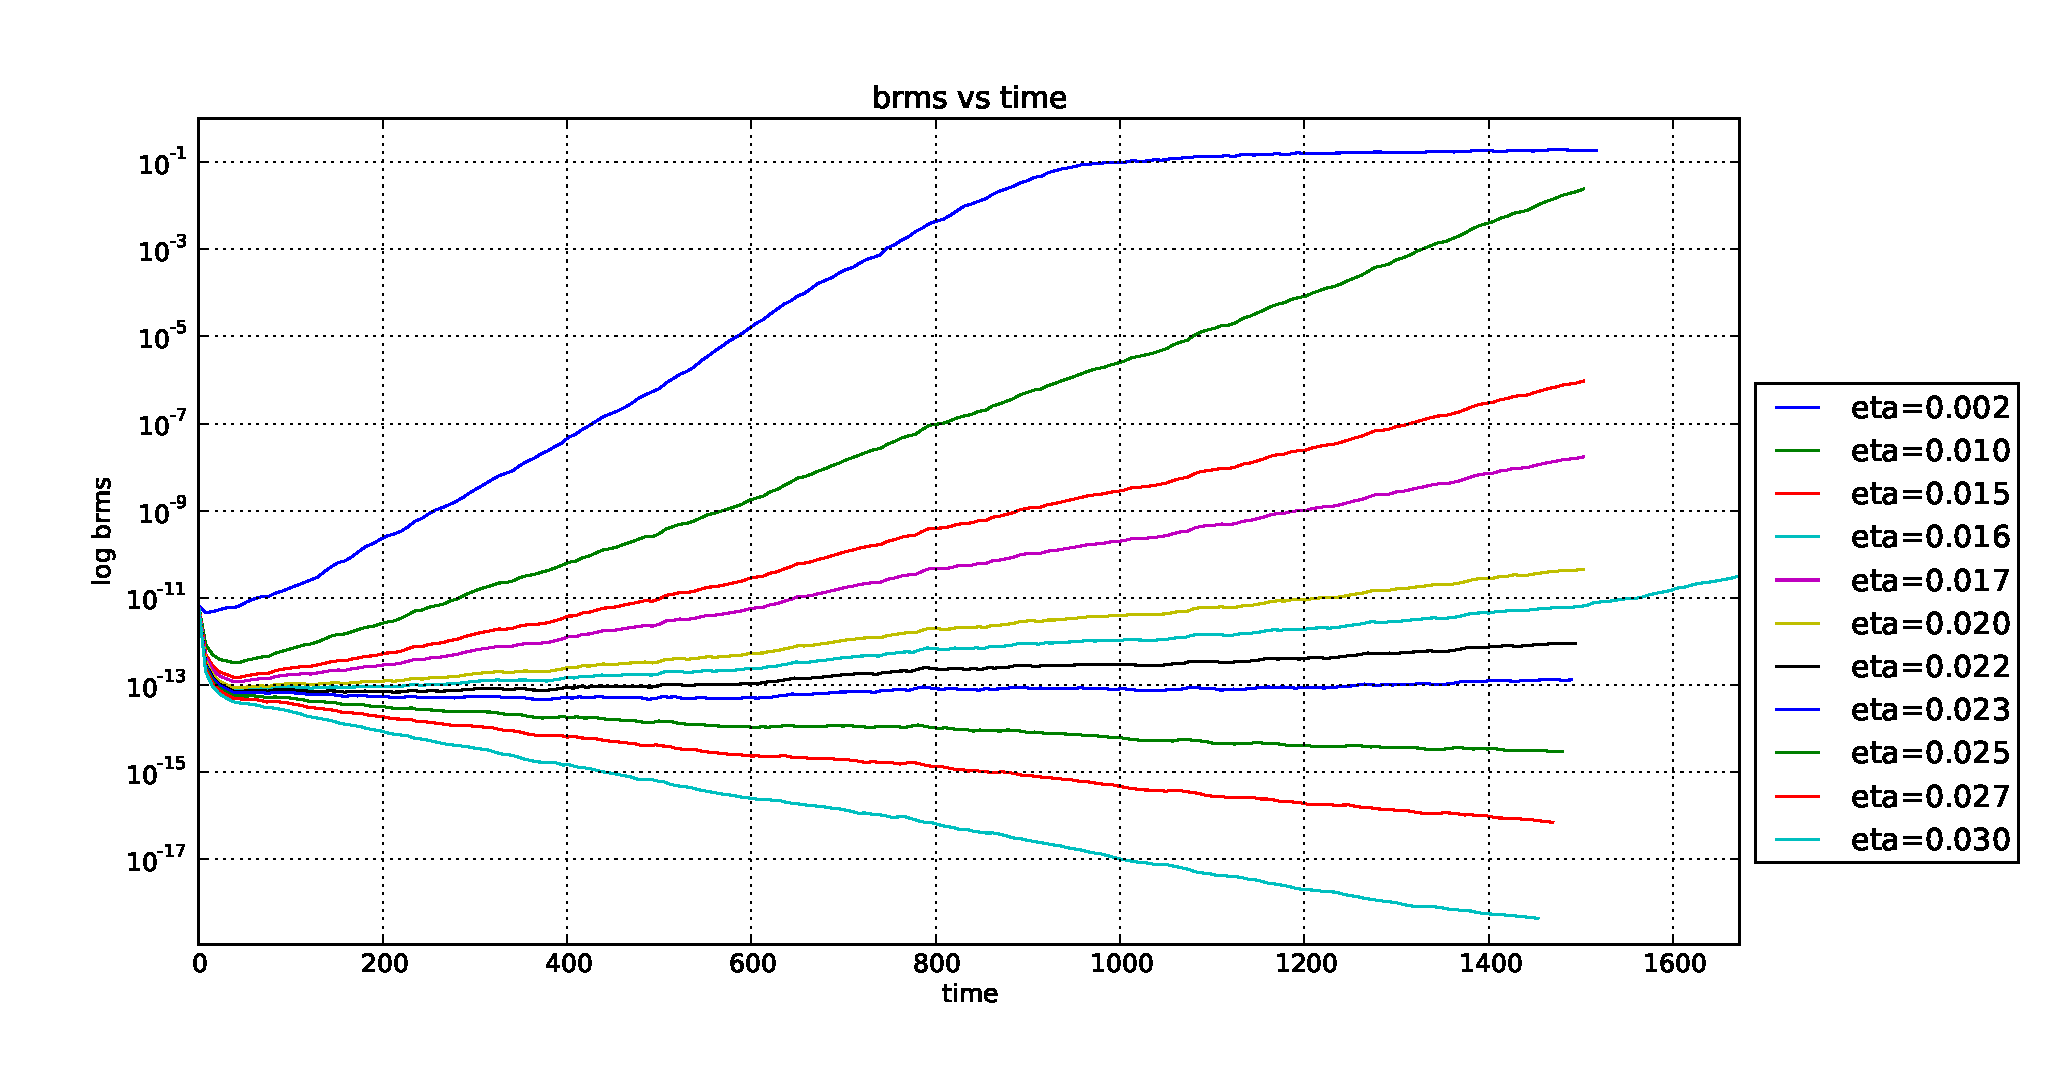
\includegraphics[width=0.8\textwidth]{brms_vs_time.eps}
\caption{log(brms) vs time for different values of  magnetic diffusivity.}
\label{fig:brmst}
 \end{figure}


I tried to find out the critical value for the magnetic diffusivity computing the first derivative of these  curves, restricted to the linear range $100 < t < 900$, and calculating the mean of each derivative. Both quantities are represented in figure \ref{fig:crit_eta}.
\begin{figure}[h]
\centering
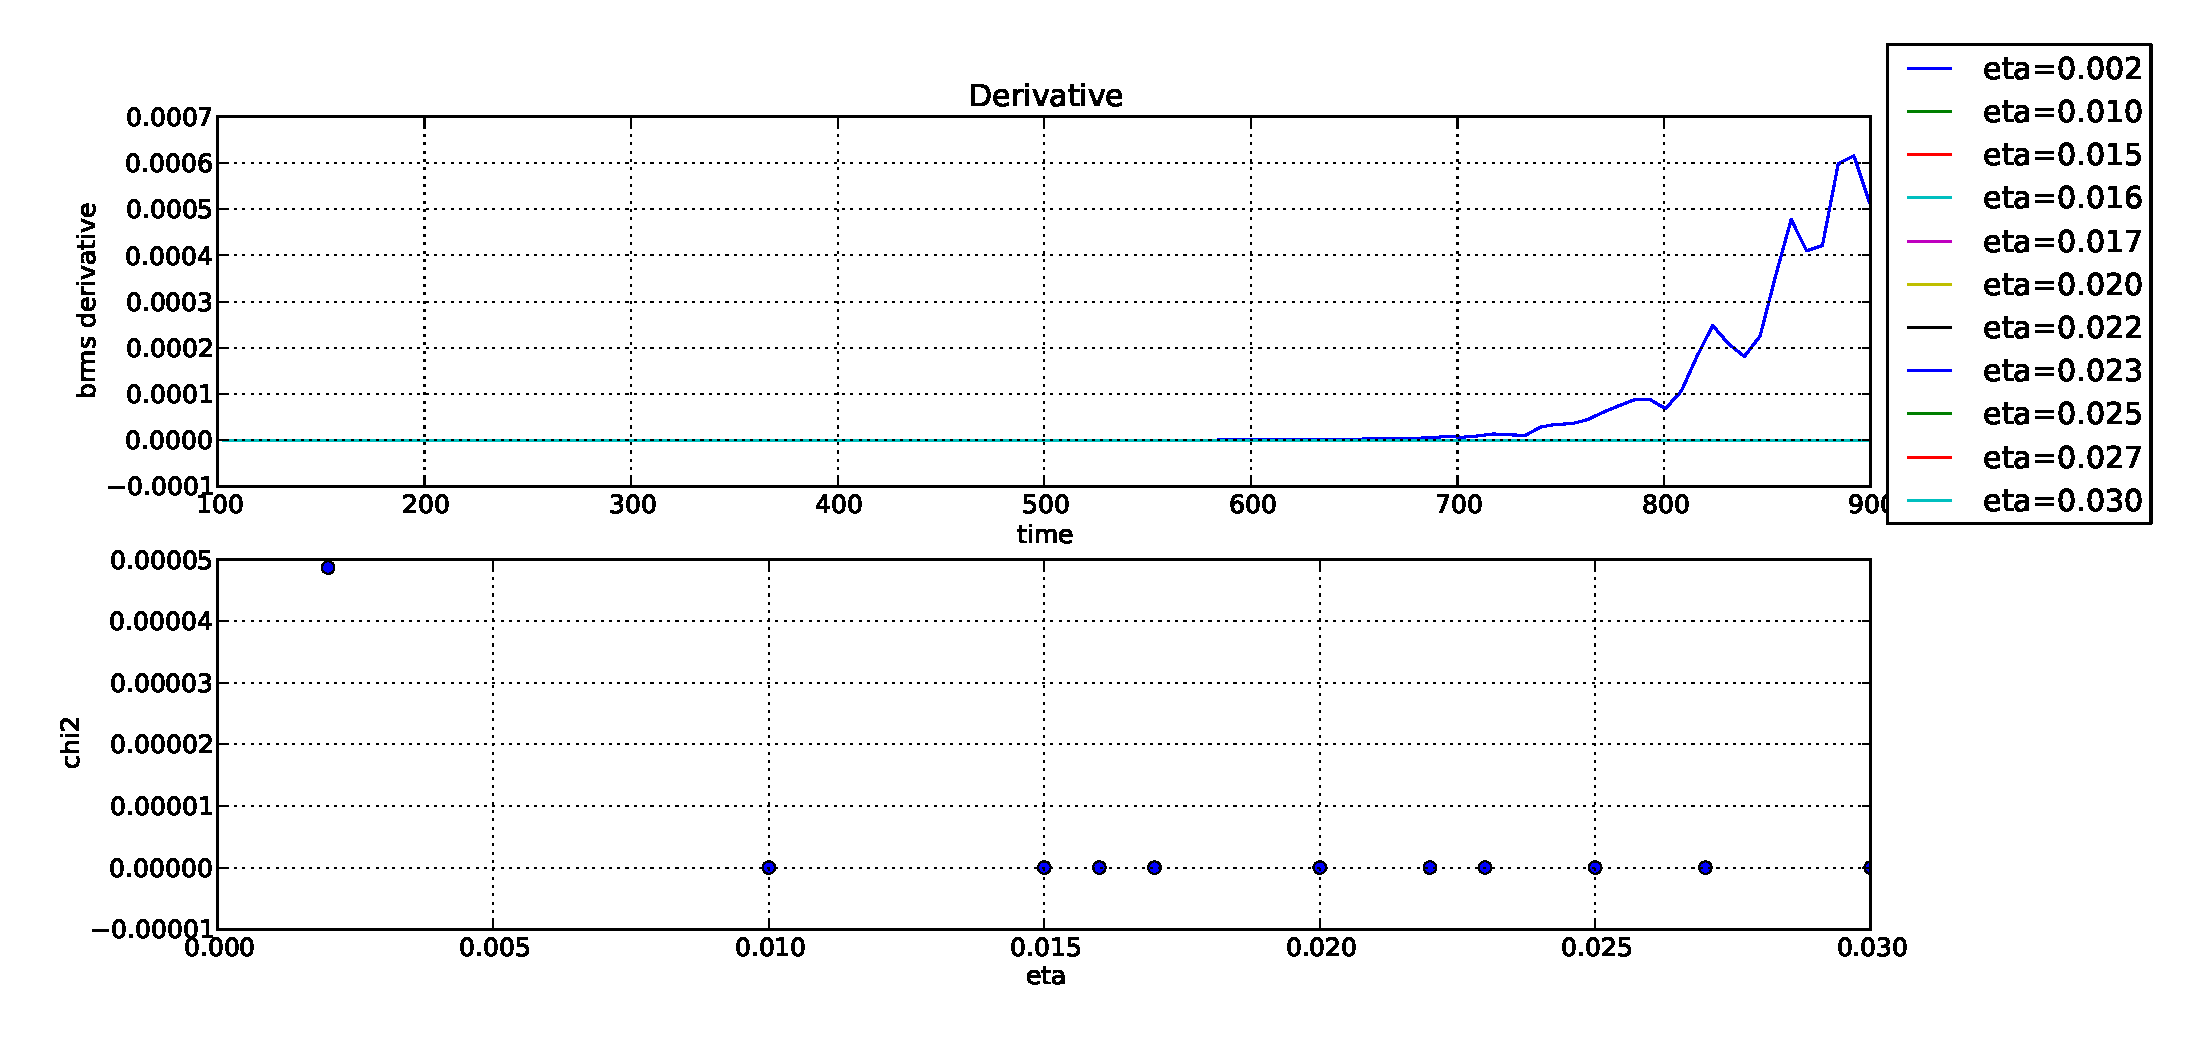
\includegraphics[width=0.8\textwidth]{critical_eta.eps}
\caption{brms derivative vs time and derivative mean for different values of the magnetic diffusivity.}
\label{fig:crit_eta}
 \end{figure}

The mean derivative of the field decreases very quickly to small values:
\begin{center}
\begin{tabular}{ll}
$\eta$ & mean(derivative)\\\hline
2e-3 & 4.87e-05\\
10e-3 & 6.89e-10\\
15e-3 & 1.48e-12\\
16e-3 & 1.04e-15\\
17e-3 & 1.33e-13\\
20e-3 & 3.63e-15\\
22e-3 & 2.63e-16\\
23e-3 & 2.52e-17\\
25e-3 & -5.09e-17\\
27e-3 & -4.54e-17\\
30e-3 & -3.07e-17\\
\end{tabular}
\end{center}

Using these results, I set the critical value for the magnetic diffusivity in $\eta = 22e-3$.

\subsection{Magnetic Reynolds number}
The magnetic Reynolds number is defined as:
\begin{equation}
 Re_M = \frac{u_{rms}}{\eta \kappa_f}
\end{equation}
In this problem I have fixed $\kappa_f = 3$, I found the critical value for the magnetic diffusivity  $\eta = 22e-3$ and the mean value for $u_{rms}$ is $\bar{u_{rms}} = 0.14$, so the corresponding magnetic Reynolds number is $Re_M = 2.15$.

The magnetic Reynolds number is the ratio between convection and diffusion. When $Re_M \gg 1$, convection dominates, whereas for $Re_M \approx 1$, or less, diffusion becomes important. So, in this exercise, diffusion is about to become important.

In fact, the next table shows that $Re_M$ decreases as $\eta$ increases:
\begin{center}
\begin{tabular}{ll}
$\eta$ & $Re_M$\\\hline
2e-3 & 22.39\\
10e-3 & 4.73\\
15e-3 & 3.16\\
16e-3 & 2.97\\
17e-3 & 2.78\\
20e-3 & 2.37\\
22e-3 & 2.15\\
23e-3 & 2.06\\
25e-3 & 1.89\\
27e-3 & 1.75\\
30e-3 & 1.58\\
\end{tabular}
\end{center}

\subsection{Growth rate of the magnetic field}

In order to determine the growth rate of the magnetic field for a value of the magnetic diffusivity, I plotted the logarithm of $brms$ versus time and I did a fit on the sloped part of the curves, as shown in the figures \ref{fig:growth2} and \ref{fig:growth10}.

\begin{figure}[h]
\begin{minipage}[t]{.45\textwidth}
\centering
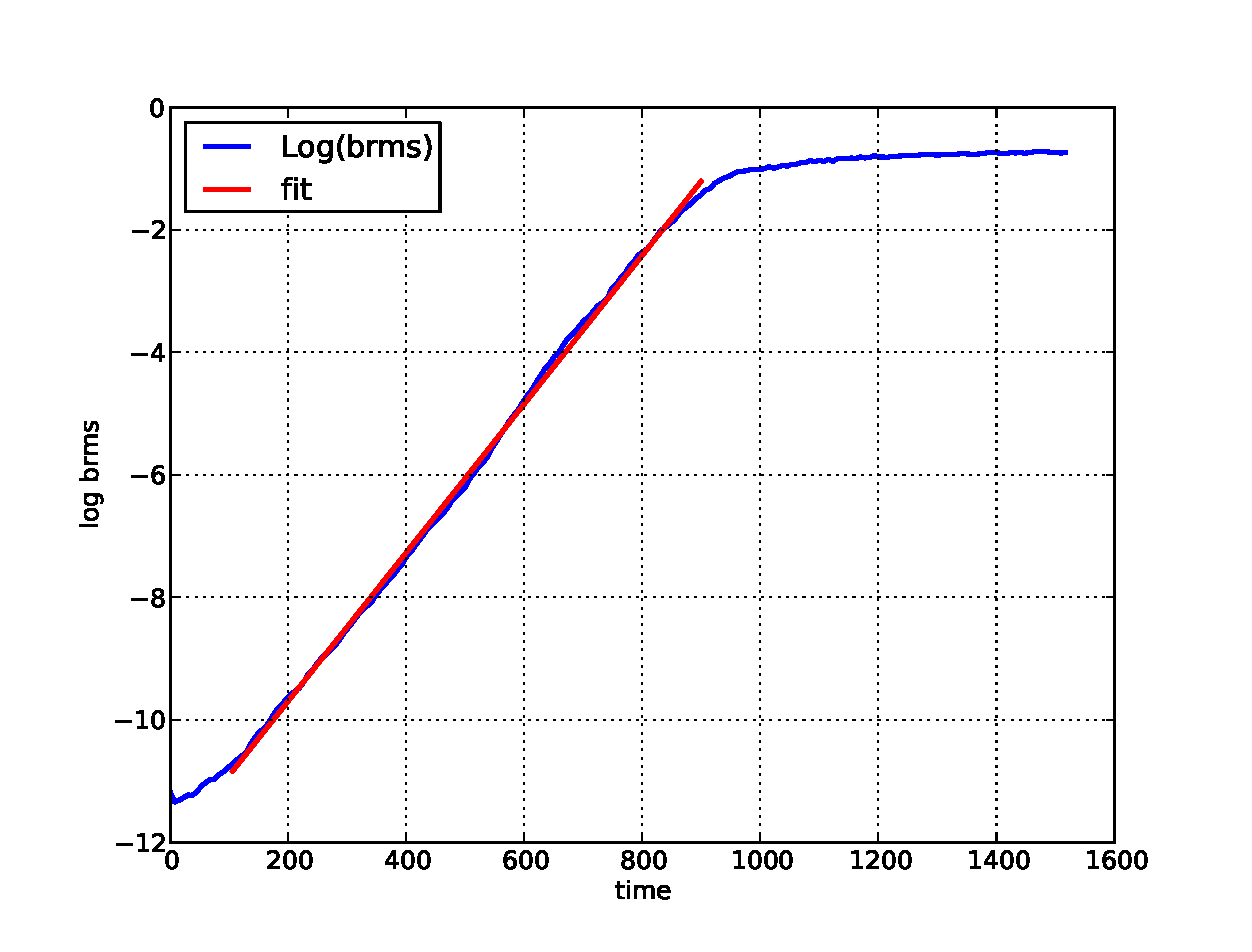
\includegraphics[width=\textwidth]{growth2e-3.eps}
\caption{Growth rate of the magnetic field for a value of the magnetic diffusivity  $\eta = 2e-3$.}
\label{fig:growth2}
\end{minipage}
\hspace{0.5cm}
\begin{minipage}[t]{.45\textwidth}
\centering
 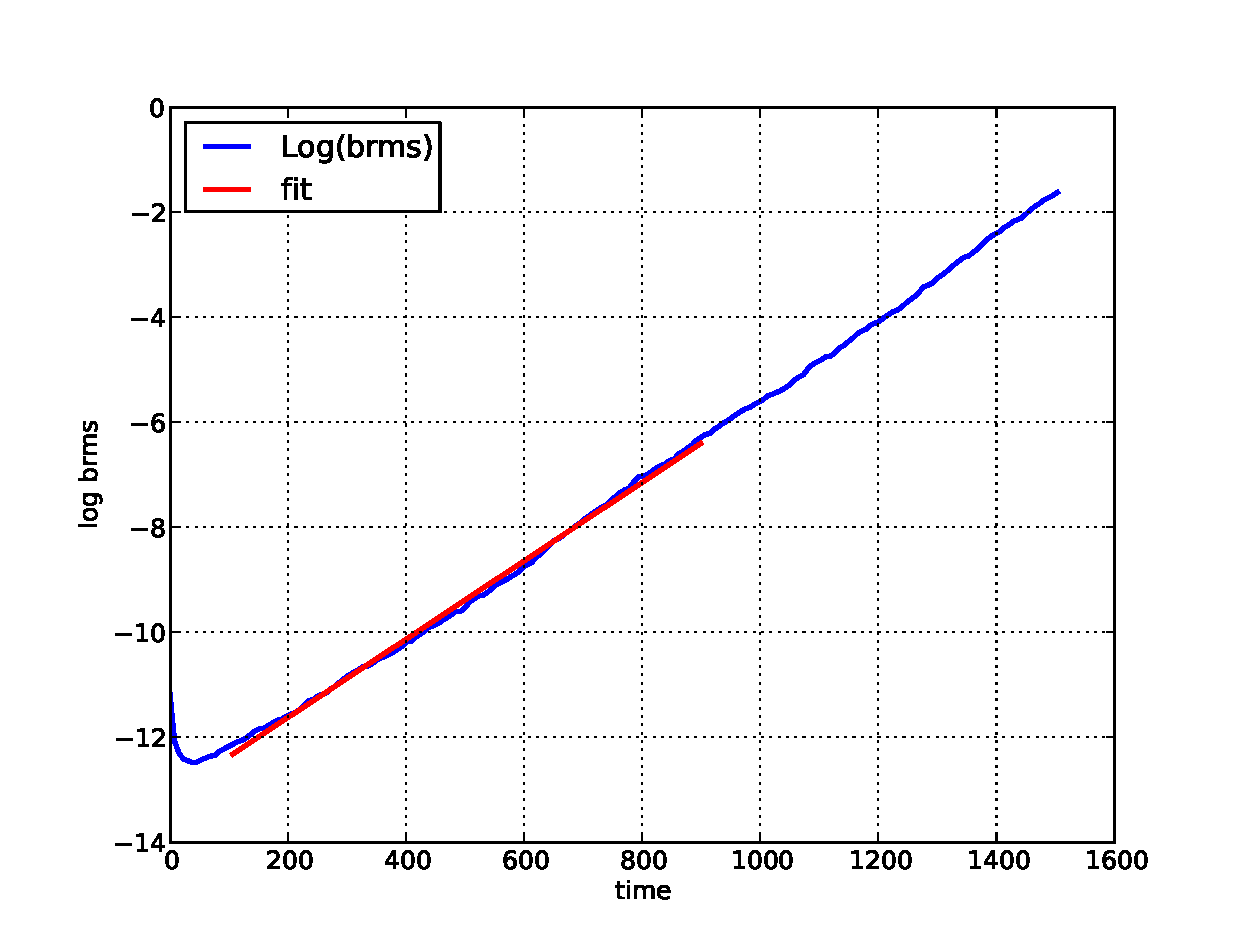
\includegraphics[width=\textwidth]{growth10e-3.eps}
\caption{Growth rate of the magnetic field for a value of the magnetic diffusivity  $\eta = 10e-3$.}
\label{fig:growth10}
\end{minipage}
 \end{figure}
%y=ax+b
The parameter $a$ in a linear regression fit ($y=ax+b$) is a measure of the growth rate of the magnetic field. The growth depends on the value of the magnetic diffusivity, and it decreases as the magnetic diffusivity increases.
\begin{center}
\begin{tabular}{lll}
$\eta$ & a & b\\\hline
2e-3 & 0.0121 & -12.12\\
10e-3 & 0.0075 & -13.11
\end{tabular}
\end{center}

\subsection{Structure of the magnetic field.}

Figure \ref{fig:averages} shows the evolution of three different magnetic field averages: the xy average bmz, the yz average bmx and the zx average bmy. 
From the figure one can see that the $zx$ average dominates in the end.
\begin{figure}[h]
\centering
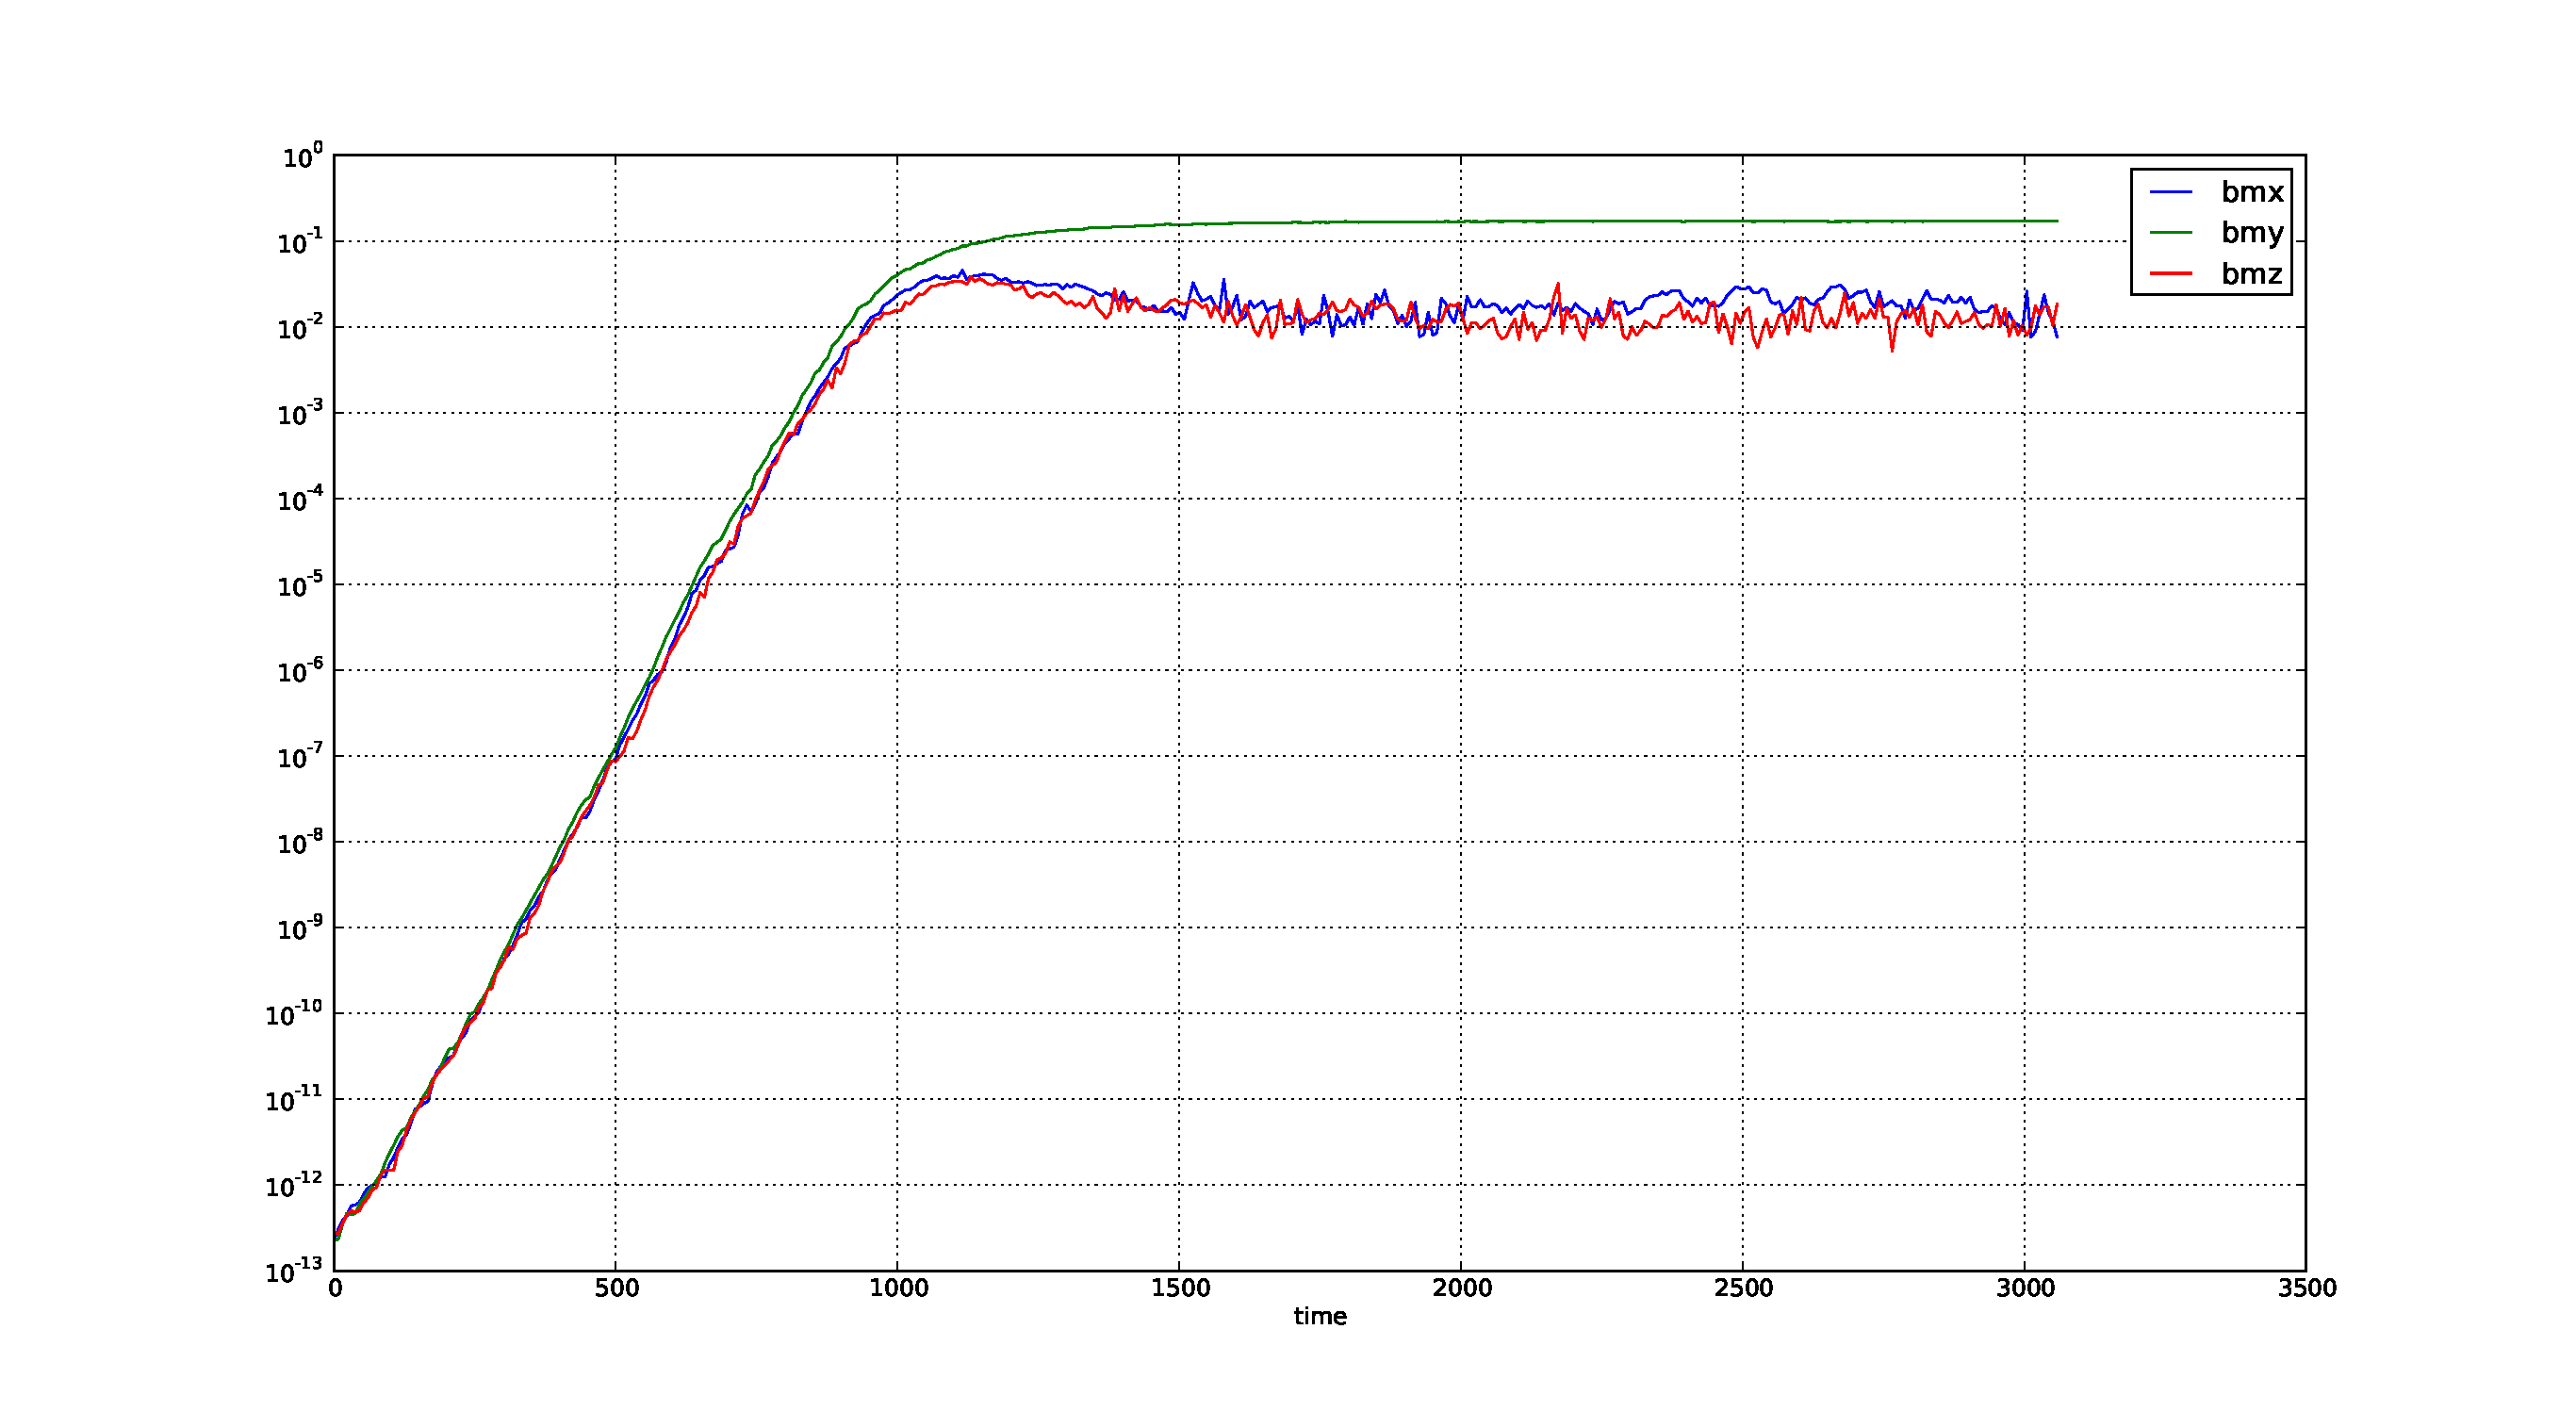
\includegraphics[width=0.8\textwidth]{campos3.eps}
\caption{Averages of three different magnetic fields.}
\label{fig:averages}
 \end{figure}

\subsection{Fitting $B_{zx}$}
Fitting the strongest of the three field averages $<\bar{B^2}>$ to the expression:
\begin{equation}
 F(t;B_0,t_s)=B_0^2[1-\exp^{-2\eta\kappa_1^2(t-t_s)}]
\label{eq:fitB}
\end{equation}
The strongest of the three field averages is the zx average represented in the figure \ref{fig:bmy_fit} with different values of the expression \ref{eq:fitB}.
\begin{figure}[h]
\centering
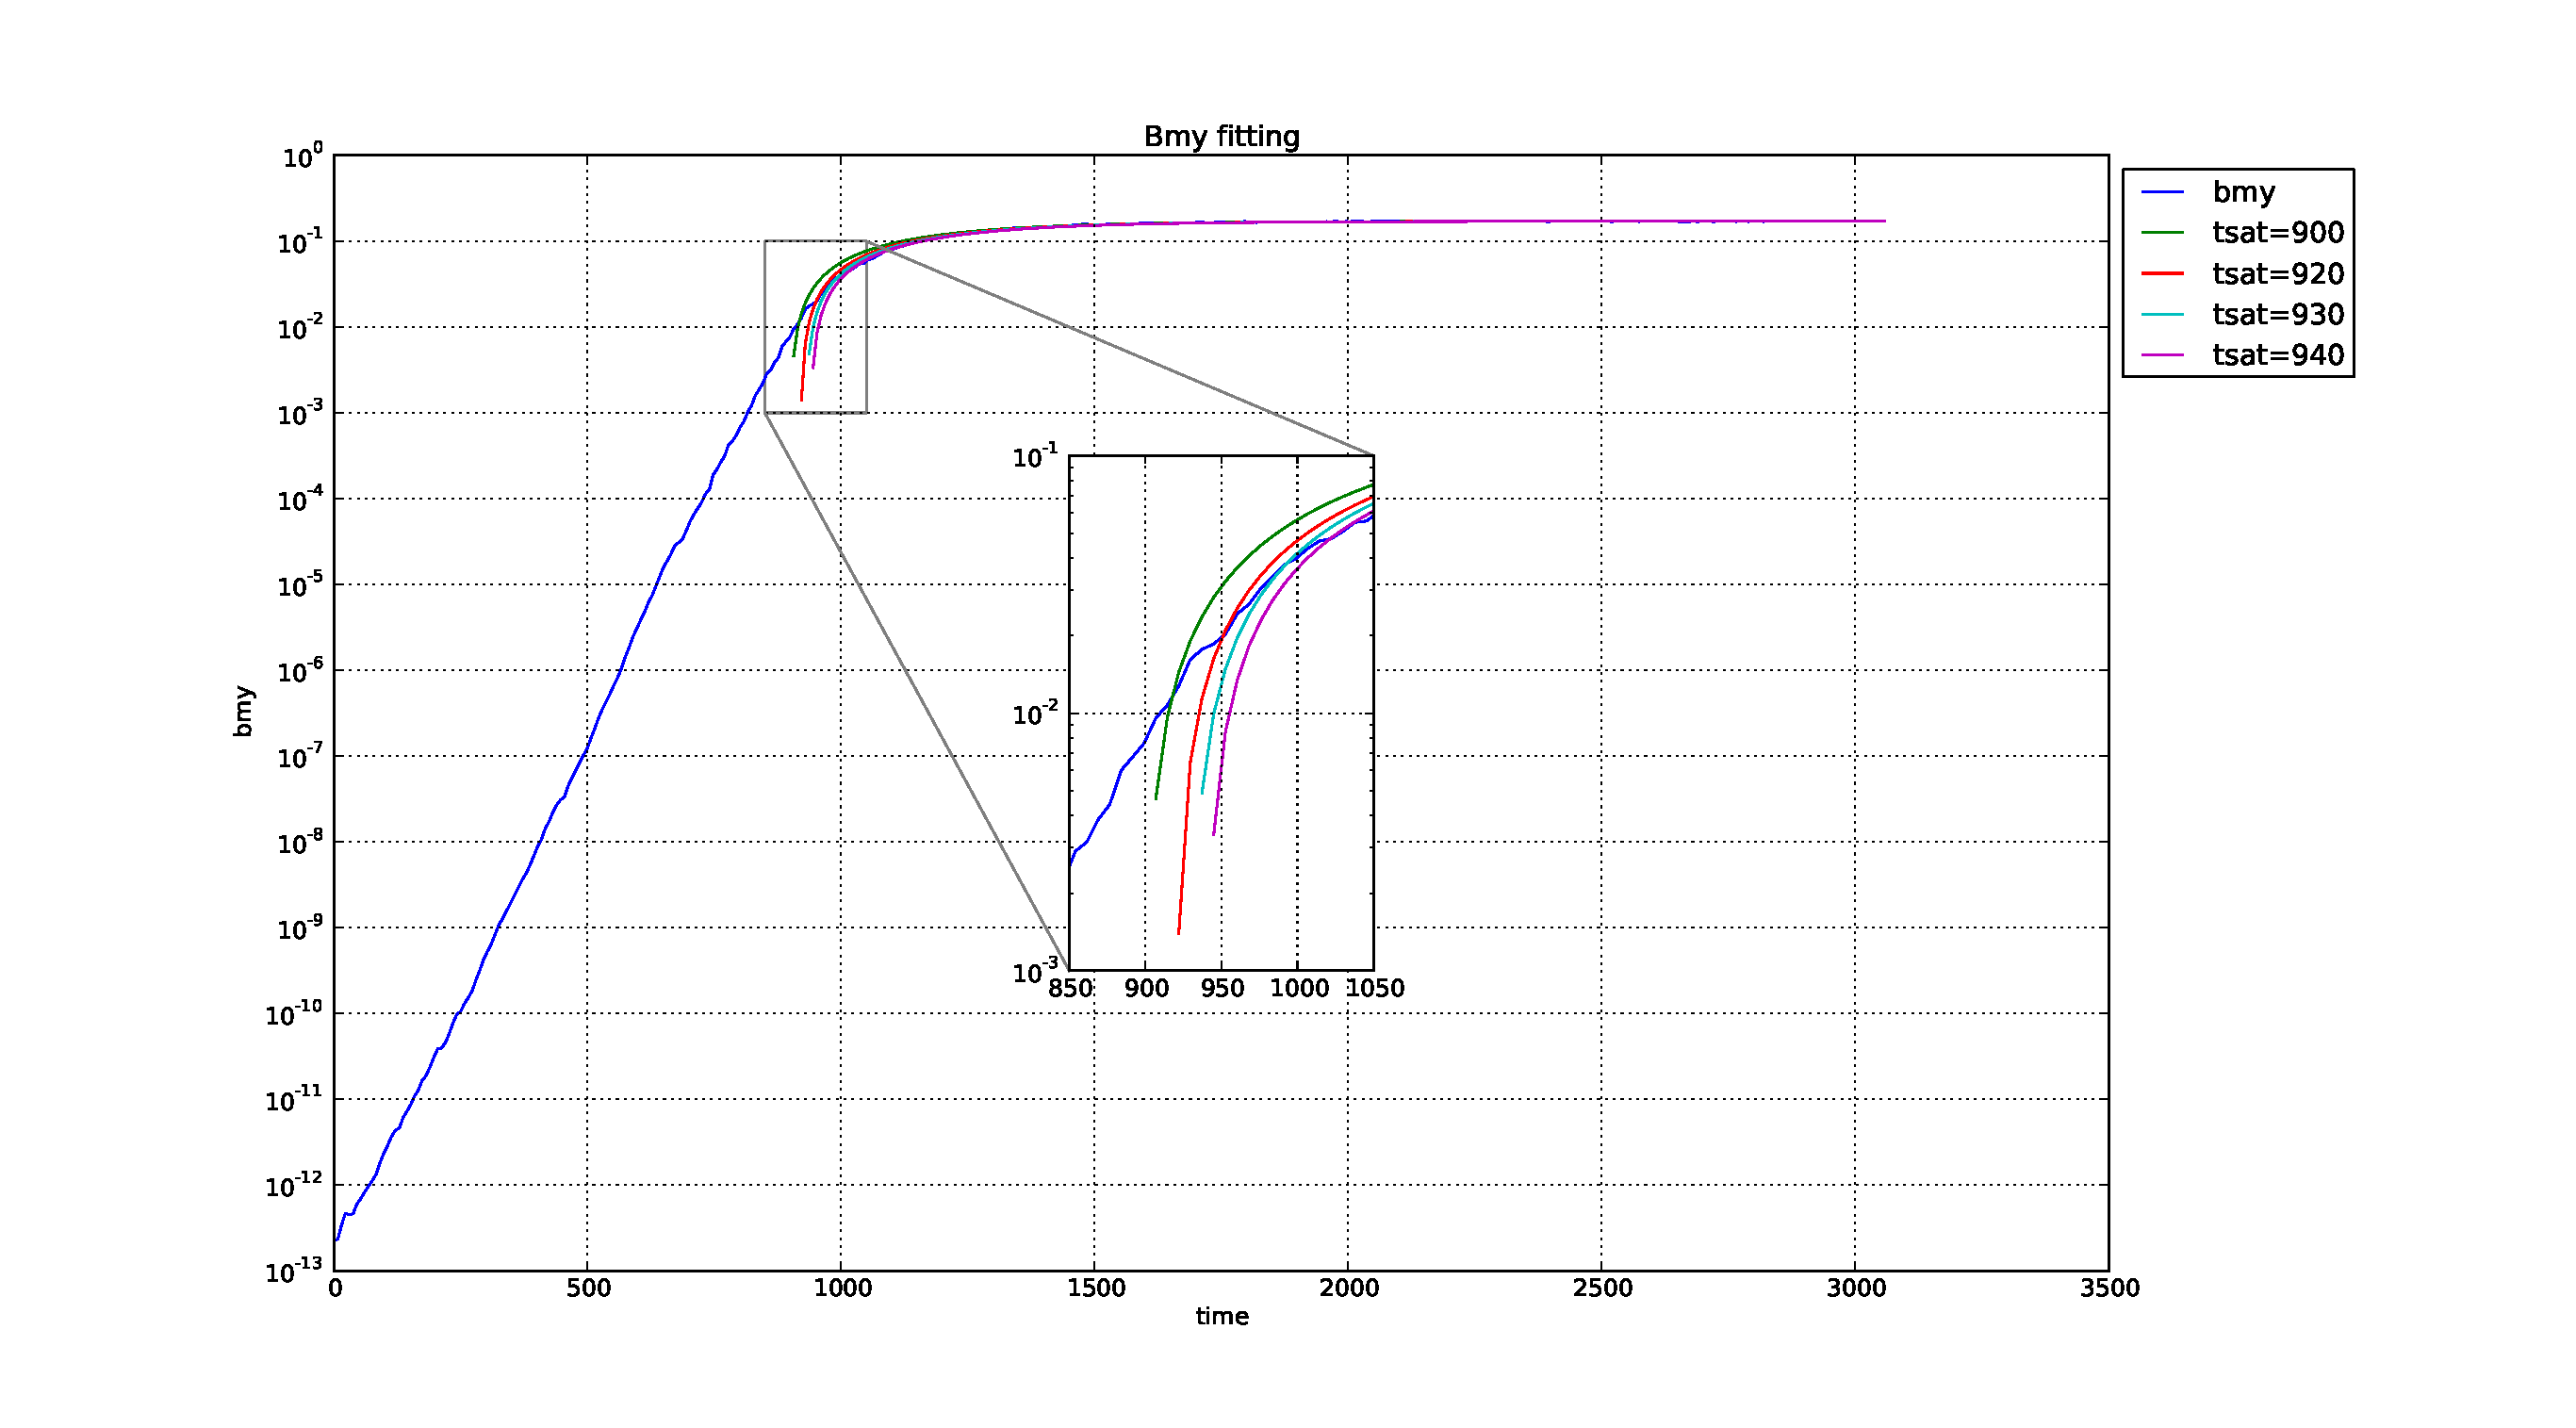
\includegraphics[width=0.8\textwidth]{bmy_fit.eps}
\caption{Bmy Fitting: $B_0=0.1712$ and $t_s = 930$.}
\label{fig:bmy_fit}
 \end{figure}
A rough fit for the field average takes the values $B_0=0.1712$ and $t_s = 930$.
$B_0$ is the saturation field value and $t_s$ is the best fit curve just before saturation.

In order to do a best mathematical fit a likelihood method could be used: 
\begin{itemize}
 \item Compute the function:
\begin{equation}
 G(t_s) = \sum_{t=a}^b (<\bar{B}^2_{(t)}>-F(t;B_0,t_s))
\end{equation}
\item Find the $t_s$ value which minimizes this function, using, for example, the false position method.

\end{itemize}



\end{document}
